% This file contains all homework from week 36
% use \section{<name>}  to create a section per homework assignment
%Andrey required packages
%\usepackage[table]{xcolor}
%\usepackage{listings}

\section[Homework 1.2]{Homework 1.2: AJAX and XML}

\subsection{History}
In early 90’s of XX century most of websites were just a plain html pages. To access recent information from the page user are required to refresh page manually. This was an inefficient method of representing information on the web. Moreover, it leads to an additional load on the server and expands the bandwidth.
\begin{itemize}
\item In 1996, Microsoft presented the first basic solution for this problem. An iframe tag was implemented in to Microsoft Internet Explorer. The iframe tag allows splitting page in to segments. Each segment contains another HTML document. The iframe standardized in HTML 4.0 Transitional and could be used in HTML5.
\item However, the iframe does not solve the problem. In 1998, the Microsoft tem firstly implemented in Outlook Web App the XMLHTTP component that client can execute by a script. 
\item In 1999, Microsoft updated the iframe technology with an XMLHTTP ActiveX object that was introduced in Internet Explorer 5. Mozilla, Safari, Opera and other browser later adopted this technology as the XMLHttpRequest JavaScript object. Later multiple web applications began to use this technology like Outlook Web App (2000), Oddpost (2002) and Gmail (2004).
\\
\item AJAX World Wide Web Consortium on 5 April 2006 published the first specification draft XMLHttpRequest object as an attempt to create an official Web standard\cite {wk01}.
\end{itemize}


\subsection{Technology}
According Jesse James Garrett, the announcer (18 February 2005) of the term Ajax (short for asynchronous JavaScript + XML):
\begin{quote}
Ajax isn’t a technology. It’s really several technologies, each flourishing in its own right, coming together in powerful new ways.\cite {jj05}
\end{quote}
Indeed Ajax consist out of the following technologies:
\begin{center}
    \begin{tabular}{l|l p{7cm}}
    \rowcolor{cyan}
    \textbf{Technology} & \textbf{Role} \\ \hline
    \rowcolor{cyan!50}
    (X)HTML and & CSS Content presentation. \\ 
    \rowcolor{cyan!10}
    DOM	& Data display and interaction. \\ 
    \rowcolor{cyan!50}
    XML	& Data interchange. \\ 
    \rowcolor{cyan!10}
    XSLT & Data manipulation. \\ 
    \rowcolor{cyan!50}
    XMLHttpRequest & Asynchronous communication. \\
    \rowcolor{cyan!10}
    JavaScript & Brings al technologies together. \\ 
    \end{tabular}
\end{center}

\subsection{Workflow}
Figure~\ref{fig:ajax} shows ajax work flow sequence\footnote{Founded on http://www.w3schools.com/ajax/ajax\_intro.asp at 10-09-2014.}: 
\begin{center}
	\begin{figure}[h!]
	  \centering
		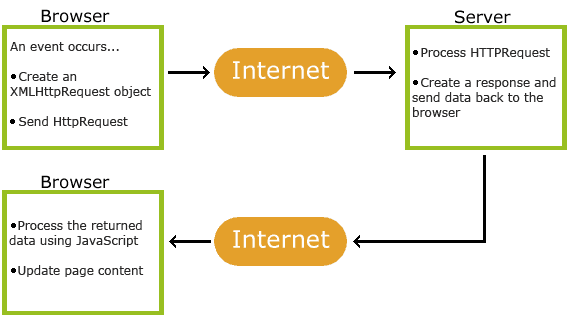
\includegraphics[scale=0.8]{ajax}
	  \caption{Ajax workflow}
	  \label{fig:ajax}
	\end{figure}
\end{center}

\newpage

\subsection{Example}
Below is an example, the comments should gave a clear picture of technologies interaction\cite{w3s}.
\lstset { %
    language=HTML,
    backgroundcolor=\color{black!5}, % set backgroundcolor
    basicstyle=\footnotesize,% basic font setting
}

\begin{lstlisting}
<! --standard  html file configuration-->
<!DOCTYPE html>
<html>
<head>
<!--Javascript-->
<script> 
function loadXMLDoc()
{
var xmlhttp;
//Definition of XMLHttpRequest object
if (window.XMLHttpRequest)
  {// code for IE7+, Firefox, Chrome, Opera, Safari
  xmlhttp=new XMLHttpRequest();
  }
else
  {// code for IE6, IE5
  xmlhttp=new ActiveXObject("Microsoft.XMLHTTP");
  }
xmlhttp.onreadystatechange=function()
  {
  if (xmlhttp.readyState==4 && xmlhttp.status==200)
    {
//Interaction with a html
    document.getElementById("myDiv").innerHTML=xmlhttp.responseText;
    }
  }
// Loading data defined in a xml file.
xmlhttp.open("GET","data.xml",true);
xmlhttp.send();
}
</script>
<!—continuing with a html -->
</head>
<body>
<h2>Unchangeable Text</h2> 
<div id="myDiv"><h2>Let AJAX change this text</h2></div>
<button type="button" onclick="loadXMLDoc()">Change Content</button>

</body>
</html>
</code>

\end{lstlisting}
\subsection{Conclusion}
Due to some difficulties with AJAX and a required asynchronous data request AJAX slightly will be replaced by JSON.
The JSON (JavaScript Object Notation), is an open standard format(RFC 7159) that uses human-readable text to transmit data objects. It is an alternative to XML and AJAX. Therefore, JSON is often used instead (see AJAJ), and the requests do not need to be asynchronous.\cite {wk02}

\newpage

\section[Homework 1.3]{Homework 1.3: XSL-FO}

In this section we describe the differences between XSLT and XSL-FO. We start by describing XSLT, XSLT is used to transform XML into some other structured format like XHTML. XSL-FO is used for formatting XML to different output formats like pdf. You can compare XSL-FO to XHTML (the structure + content) and CSS (the styling). See figure \ref{fig:XSL}.

\begin{figure}[H]
	\centering
	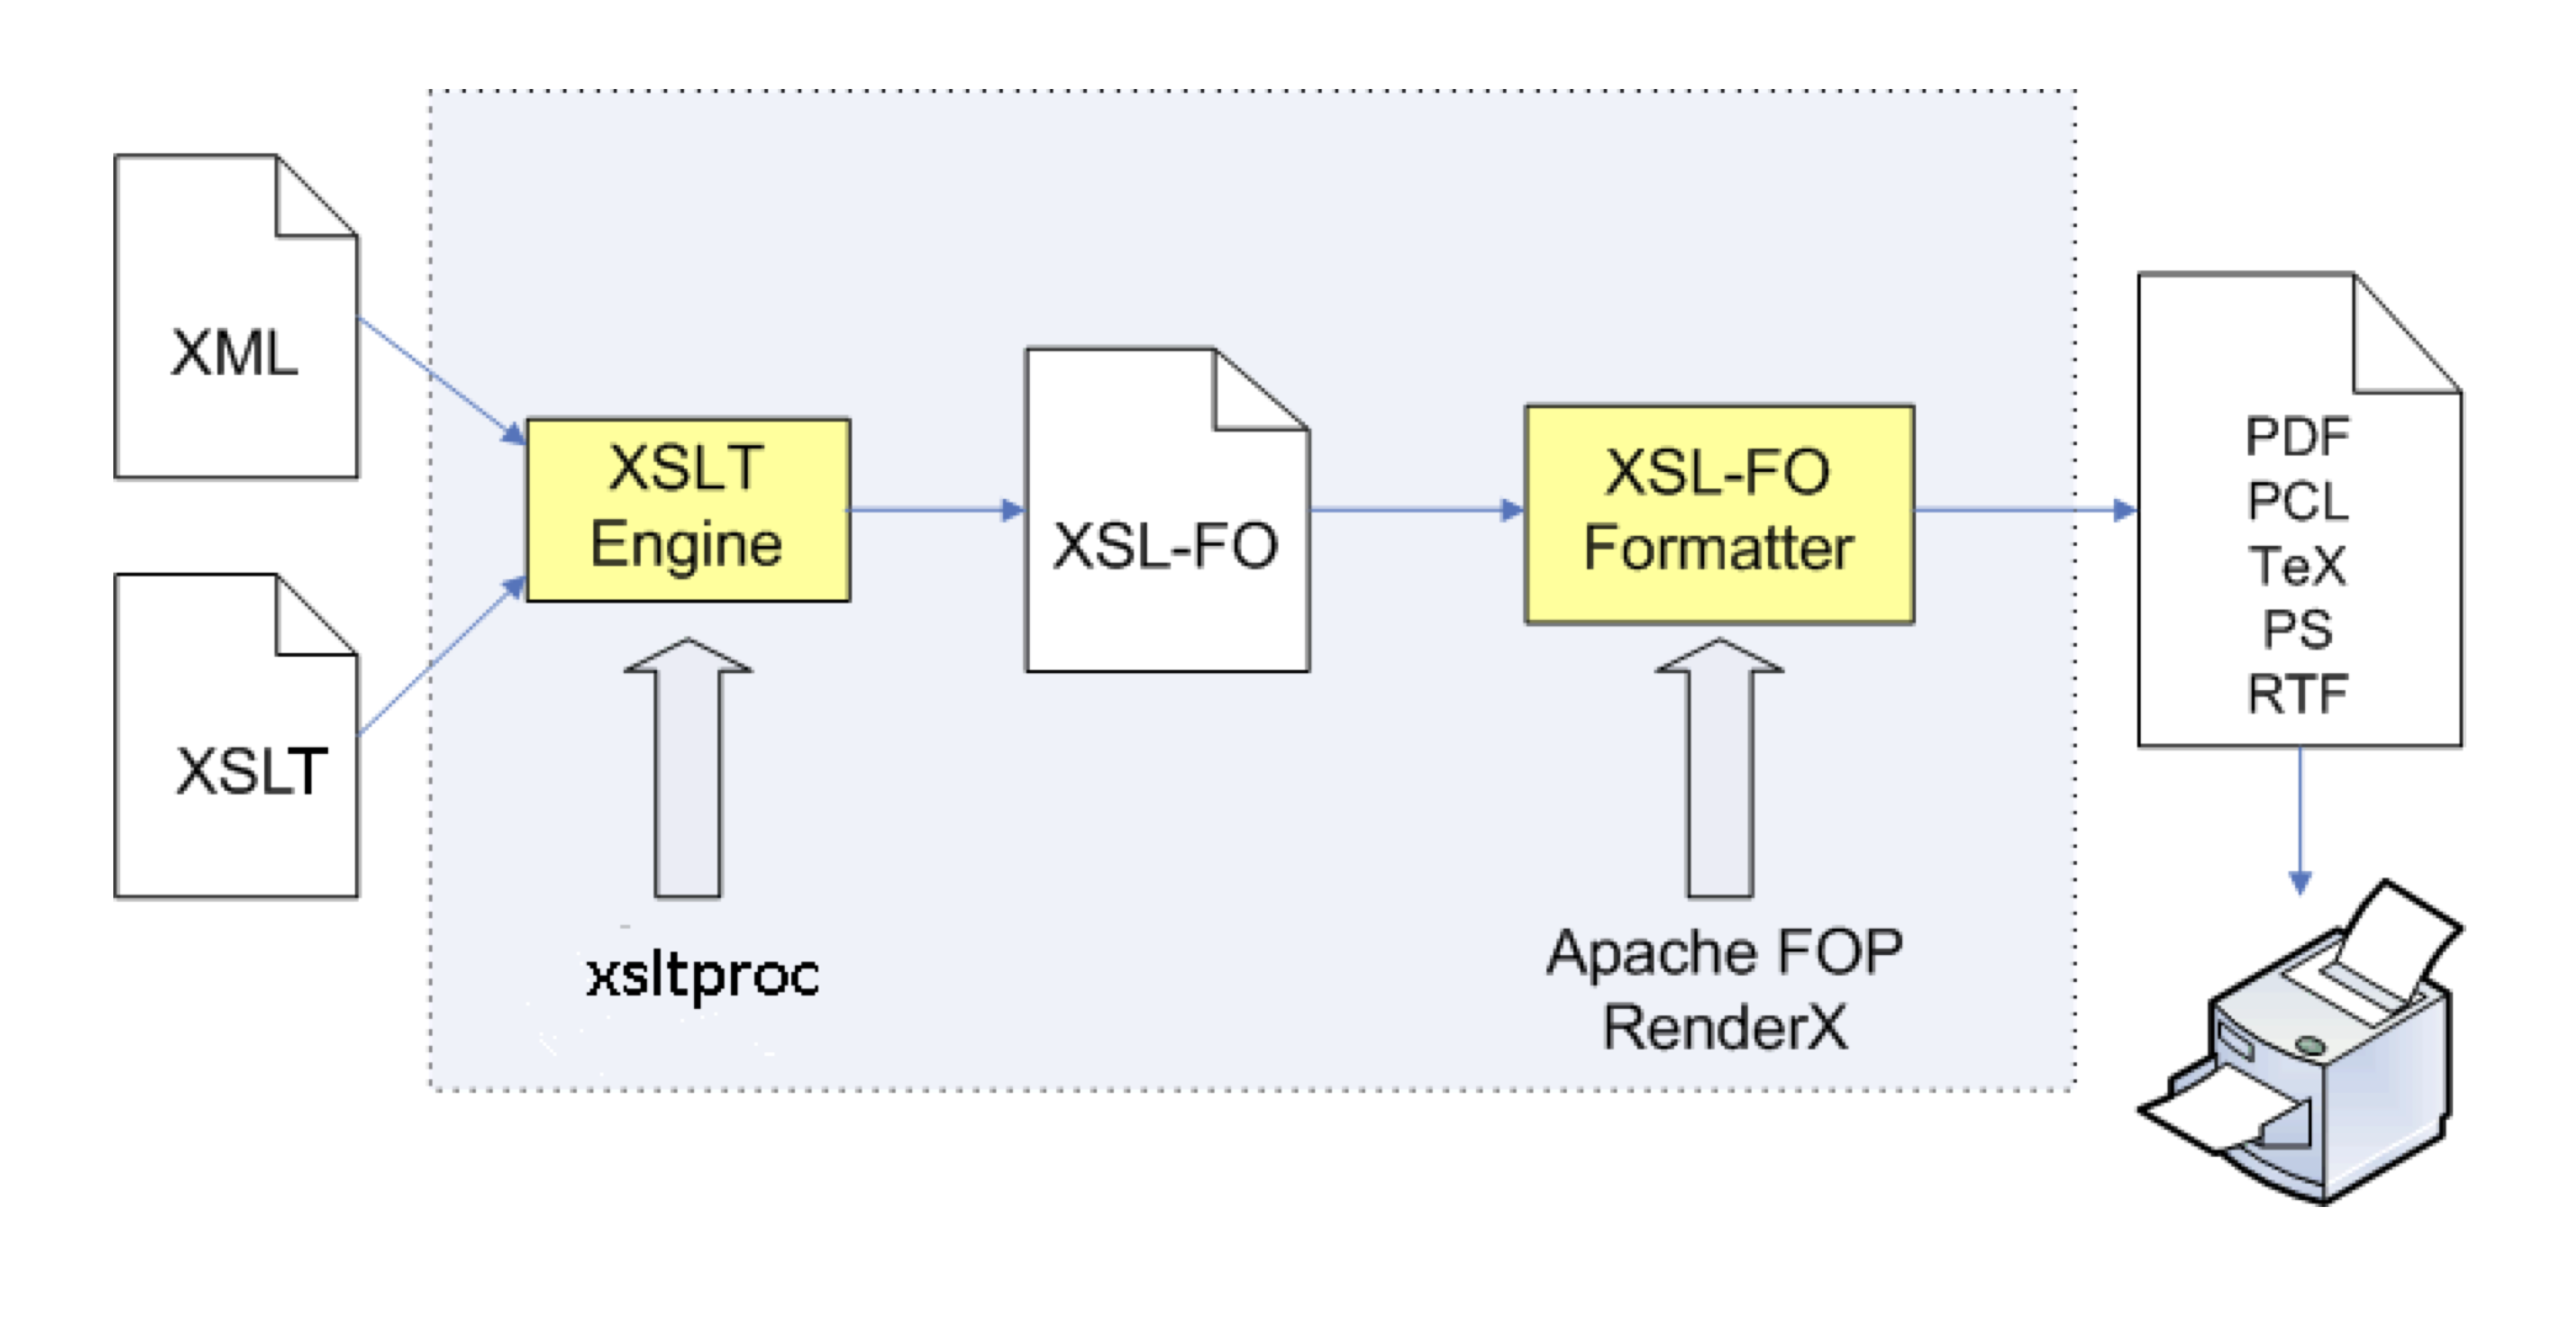
\includegraphics[scale=1.3]{XSL_FO}
	\caption{This figure shows the transformation from XML using XSLT and XSL-FO to some output format adapted from \cite{XSL-FO}}
	\label{fig:XSL}
\end{figure}
